\documentclass{article}

\usepackage[margin = 1in]{geometry}
\usepackage{minted}
\usepackage{amsmath}
\usepackage{amssymb}
\usepackage{graphicx}
\usepackage{subcaption}
\usepackage{xcolor}
\usepackage{setspace}
\usepackage{hyperref}
\usepackage[backend=biber]{biblatex}

\bibliography{project-report.bib}
\doublespacing

\title{Final Project Report}
\author{Leanna Calla \\ Michael Stergianis}
\date{March 27th, 2018}

\newcommand{\norm}[1]{\left\| #1 \right\|}

\begin{document}
\maketitle
%
\section{Introduction}
\begin{flushleft}
  %
  When attempting to increase the detail of an image, any noise in
  that image will also be used in the interpolation scheme. Therefore
  an integral first step to super resolution is to denoise the image
  in a way that preserves edges, corners, and the finer details of the
  image.
  %
\end{flushleft}
%
\section{Filtering Techniques}

%\begin{flushleft}


\subsection{Gaussian Blur}
As described in \cite{bilateral}, Gaussian blur is a linear filtering
technique which takes local averages of pixel intensities. The
Gaussian blurred image is defined as follows
\[GB[I]_p = \displaystyle \sum_{\textbf{q} \in S}G_{\sigma} \left(
    \norm{\textbf{p} - \textbf{q}}\right)I_{\textbf{q}} \]
where the two dimensional Gaussian kernel, $G_{\sigma}(x)$ is given by
\[G_{\sigma}(x) = \frac{1}{2 \pi \sigma^2} \text{exp} \left(-
    \frac{x^2}{2 \sigma^2}\right). \]

\subsection{Bilateral Filter}
The Bilateral filter as given in \cite{Faisal-bilateral} is as follows

\[ BF[I]_{\textbf{p}}= \displaystyle \sum_{\textbf{q} \in S} G_{\sigma_s} \left(\norm{\textbf{p} - \textbf{q}}\right) G_{\sigma_r} \left(|I_{\textbf{p}} - I_{\textbf{q}}|\right)I_{\textbf{q}} \]
Where the Gaussian blur term is used as a space weight, and the
additional term in the sum is the range weight. Note, the sum has also
been normalized. This filtering technique takes into account the
effects of space and range parameters. The space parameter,
$\sigma_s$, refers to the spatial extent of the kernel. The Gaussian
over this element will decrease the influence of distant pixel. The
range parameter, $\sigma_r$, refers to the minimum amplitude of an
edge. The Gaussian over this parameter will decrease the intensity of
pixels whose value is different from $I_{\textbf{p}}$. The bilateral
filter tends to break the image into two layers. \cite{bilateral}
describes the layers as a large layer which is a smoother version of
the image with the contours preserved and a smaller layer which can be
thought of as the residual of the image, which may contain noise or
texture. The bilateral filter smooths an image while preserving the
image's discontinuities. 
%\end{flushleft}
\subsection{Median Filtering}
%
\begin{flushleft}
  %
  Median filtering is a common technique to remove noise from an
  image. \cite{Med2012} explores the median filter. A median filter is a
  nonlinear filter. A sliding mask is applied to the image, where the
  value of a noisy pixel is replaced by the median of the pixels in
  the mask. The performance of the median filter depends on the size
  of the mask and the distribution of the noise.

  \subsection{Improved Median}
   \cite{improved-median} and \cite{Med2012} shows progress on an
   improved median filter over a year. The algorithm
   \texttt{improved\_median} has been implemented to show the improved
   filtering techniques as suggested by the papers. The improved
   median filter compared with
   the standard median filter in the Statistics section. The steps of
   the improved median filter algorithm are as
   follows
   \begin{enumerate}
   \item an $n\times n$ mask is chosen to slide over the image
     \item the median, \textit{median}, of the mask is computed. This
       is done by ordering the elements and choosing the middle
       element as the median
       \item a new average is computed, \textit{avg}. In this average the
         central element is replaced with \textit{median}.
         \item Each pixel in the mask is compared with
           \textit{avg}
           \item if every pixel in the mask is greater than the
             \textit{avg}, then the central pixel is replaced with the
             median of the patch
           \item otherwise the patch is unchanged
             \item steps 4-6 will be repeated until the image has been
               completely traversed.
     \end{enumerate}
   
  \end{flushleft}
%
  \section{Interpolation Techniques}
  
  %
  \section{Testing Code}
  A data set was created with a Matlab script. Two of Matlab's images,
  \texttt{cameraman.tif} and \texttt{peppers.png} were used. Noise was
  added to these images in four different ways. The noisy images are
  shown in figure 1 and 2. The following filters
  were applied
  \begin{itemize}
    \item salt and pepper noise, with the default settings, with
      default noise density of 0.05
    \item gaussian noise, with default adding zero mean and variance
      of 0.01 
    \item speckle noise, with defaults adding random noise with mean 0
      and variance 0.04 
    \item poisson noise, default settings generate Poisson noise from
      the data
    \end{itemize}

    \begin{figure}[H]
      \centering
      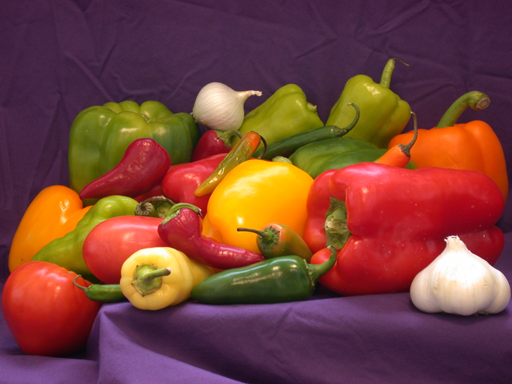
\includegraphics[width =0.15\textwidth]{../images/peps_truth}
      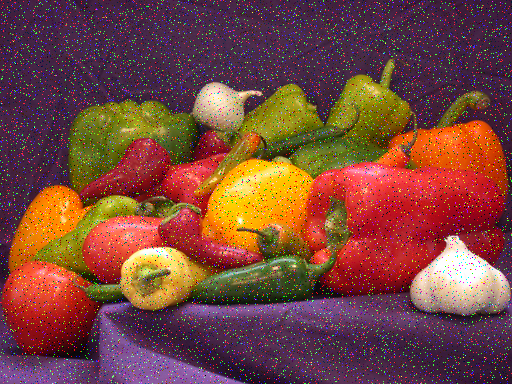
\includegraphics[width =0.15\textwidth]{../images/peps_noisy1}
      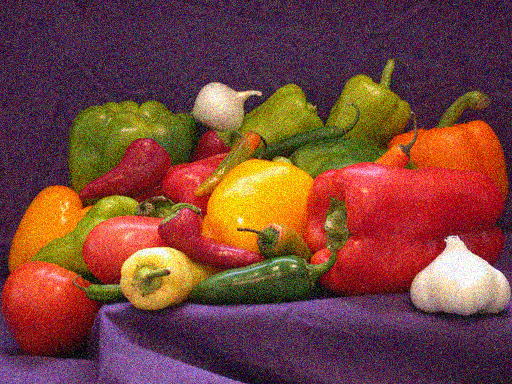
\includegraphics[width =0.15\textwidth]{../images/peps_noisy2}
      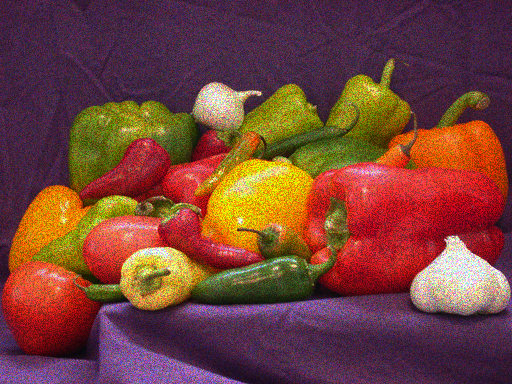
\includegraphics[width =0.15\textwidth]{../images/peps_noisy3}
      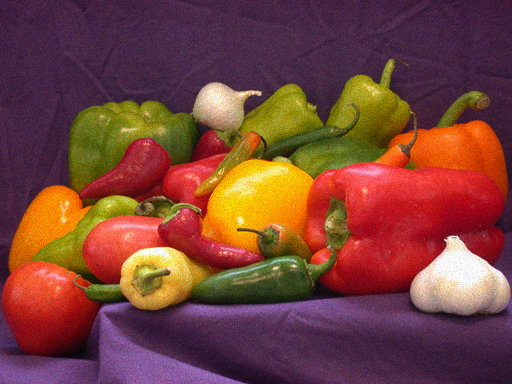
\includegraphics[width =0.15\textwidth]{../images/peps_noisy4}
      \caption{Ground truth displayed first, followed by the noisy
        images ordered by the filters as given above}
    \end{figure}
    
 \begin{figure}[H]
      \centering
      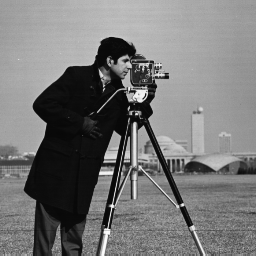
\includegraphics[width =0.15\textwidth]{../images/camera_truth}
      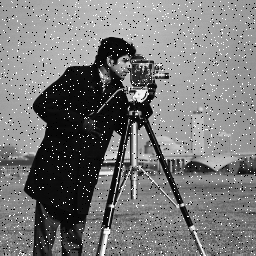
\includegraphics[width =0.15\textwidth]{../images/camera_noisy1}
      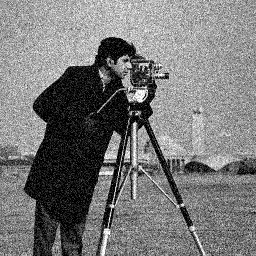
\includegraphics[width =0.15\textwidth]{../images/camera_noisy2}
      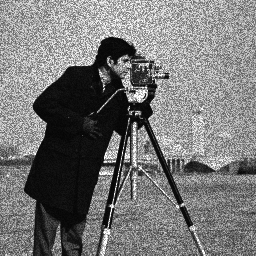
\includegraphics[width =0.15\textwidth]{../images/camera_noisy3}
      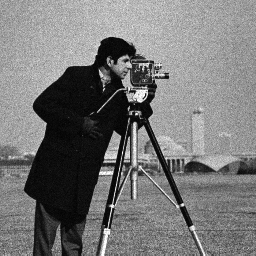
\includegraphics[width =0.15\textwidth]{../images/camera_noisy4}
      \caption{Ground truth displayed first, followed by the noisy
        images ordered by the filters as given above}
    \end{figure}   

  \section{Statistics Tracking}
  %
  Three different denoising techniques have been applied to the
  figures. Signal to noise ratios (snr) and root mean
  square errors (rmse) have been computed to show the effectiveness of each
  filtering technique.
  %
  \subsection{Gaussian Denoising}
  The Gaussian technique as described in section 2.1 has been applied
  to the noisy images. The resulting images are seen in figure 3 and 4.
  \subsubsection{Performance on colour image - peppers}
  \begin{figure}[H]
      \centering
      \includegraphics[width
      =0.2\textwidth]{../../denoised/peps_noisy1_gaussian}
      \includegraphics[width
      =0.2\textwidth]{../../denoised/peps_noisy2_gaussian}
      \includegraphics[width
      =0.2\textwidth]{../../denoised/peps_noisy3_gaussian}
      \includegraphics[width =0.2\textwidth]{../../denoised/peps_noisy4_gaussian}
      \caption{Gaussian filter applied to all four noisy images }
    \end{figure}
    \begin{tabular}{|c|c|c|c|c|}
      \hline
      \multicolumn{5}{|c|}{Image Statistics - Performance of Gaussian blur}\\
    \hline
    \hline
      & salt \& pepper noise & gaussian noise&speckle noise & poisson noise\\
      \hline
      snr & 0.3062540126612596 &0.2583390404539884  & 0.25708580687724447  &  0.2721887912258063\\
      \hline
      rmse &  0.31783307329595933 & 0.3647440957521513 & 0.33988432669381763 &  0.29706777764981346 \\
      \hline

    \end{tabular}


    \subsubsection{Performance on grayscale image - cameraman}
  \begin{figure}[H]
      \centering
      \includegraphics[width
      =0.2\textwidth]{../../denoised/camera_noisy1_gaussian}
      \includegraphics[width
      =0.2\textwidth]{../../denoised/camera_noisy2_gaussian}
      \includegraphics[width
      =0.2\textwidth]{../../denoised/camera_noisy3_gaussian}
      \includegraphics[width =0.2\textwidth]{../../denoised/camera_noisy4_gaussian}
      \caption{Gaussian filter applied to all four noisy images }
    \end{figure}
    \begin{tabular}{|c|c|c|c|c|}
      \hline
      \multicolumn{5}{|c|}{Image Statistics - Performance of Gaussian blur}\\
    \hline
    \hline
      & salt \& pepper noise & gaussian noise &speckle noise & poisson noise\\
      \hline
      snr & 0.17488795783381422 & 0.2671556265312336 & 0.44244029168868537 & 0.2648366712931854 \\
      \hline
      rmse &0.1895823535533745  &  0.2098089541648092 &  0.18415594753856307 & 0.16077582960772\\
      \hline
    \end{tabular}


    \subsection{Median Denoising}
    The median filter as described in 2.3 was applied to the set of
    noisy images. Results can be seen in figures 5 and 6.
    \subsubsection{Performance on colour image - peppers}
 \begin{figure}[H]
      \centering
      \includegraphics[width
      =0.2\textwidth]{../../denoised/peps_noisy1_median}
      \includegraphics[width
      =0.2\textwidth]{../../denoised/peps_noisy2_median}
      \includegraphics[width
      =0.2\textwidth]{../../denoised/peps_noisy3_median}
      \includegraphics[width =0.2\textwidth]{../../denoised/peps_noisy4_median}
      \caption{Median filter filter applied to all four noisy images }
    \end{figure}
    \begin{tabular}{|c|c|c|c|c|}
      \hline
      \multicolumn{5}{|c|}{Image Statistics - Performance of Median filtering}\\
    \hline
    \hline
      & salt \& pepper noise & gaussian noise &speckle noise & poisson noise\\
      \hline
      snr & 0.028134497955144933 & 0.03591899383833425 & 0.13359570054045616& 0.055596194981823936\\
      \hline
      rmse & 0.19619888890010365 &  0.22255589087006272 &  0.21299238333129938  &0.20900209235717904 \\
      \hline
    \end{tabular}

     \subsubsection{Performance on grayscale image - cameraman}
  \begin{figure}[H]
      \centering
      \includegraphics[width
      =0.2\textwidth]{../../denoised/camera_noisy1_median}
      \includegraphics[width
      =0.2\textwidth]{../../denoised/camera_noisy2_median}
      \includegraphics[width
      =0.2\textwidth]{../../denoised/camera_noisy3_median}
      \includegraphics[width =0.2\textwidth]{../../denoised/camera_noisy4_median}
      \caption{Median filter applied to all four noisy images }
    \end{figure}
    \begin{tabular}{|c|c|c|c|c|}
      \hline
      \multicolumn{5}{|c|}{Image Statistics - Performance of median filtering}\\
    \hline
    \hline
      & salt \& pepper noise & gaussian noise &speckle noise & poisson noise\\
      \hline
      snr & 0.08315701668985512  & 0.08410367208570518  &0.14337351728292427   & 0.09863654556279272  \\
      \hline
      rmse & 0.34980467051384057 & 0.3874309974622892  & 0.37596914471909365 & 0.37580375518905496\\
      \hline
    \end{tabular}



    \subsection{Improved Median Denoising}
    The algorithm is proposed by \cite{improved-median} and
    \cite{Med2012} has been applied to the noisy images. Results found
    in figures 7 and 8.
    \subsubsection{Performance on colour image - peppers}
 \begin{figure}[H]
      \centering
      \includegraphics[width
      =0.2\textwidth]{../../denoised/peps_noisy1_improved_median}
      \includegraphics[width
      =0.2\textwidth]{../../denoised/peps_noisy2_improved_median}
      \includegraphics[width
      =0.2\textwidth]{../../denoised/peps_noisy3_improved_median}
      \includegraphics[width =0.2\textwidth]{../../denoised/peps_noisy4_median}
      \caption{Median filter filter applied to all four noisy images }
    \end{figure}
    \begin{tabular}{|c|c|c|c|c|}
      \hline
      \multicolumn{5}{|c|}{Image Statistics - Performance of Improved Median filtering}\\
    \hline
    \hline
      & salt \& pepper noise & gaussian noise &speckle noise & poisson noise\\
      \hline
      snr & -0.4544166729015866 & -0.1760805296664718 &0.05383791460923117 & 0.008529101964318823\\
      \hline
      rmse &  0.03494201787954231 &  0.21491019365990058 &  0.21598442221428243  & 0.2176207971318631 \\
      \hline
    \end{tabular}

     \subsubsection{Performance on grayscale image - cameraman}
  \begin{figure}[H]
      \centering
      \includegraphics[width
      =0.2\textwidth]{../../denoised/camera_noisy1_improved_median}
      \includegraphics[width
      =0.2\textwidth]{../../denoised/camera_noisy2_improved_median}
      \includegraphics[width
      =0.2\textwidth]{../../denoised/camera_noisy3_improved_median}
      \includegraphics[width =0.2\textwidth]{../../denoised/camera_noisy4_improved_median}
      \caption{Median filter applied to all four noisy images }
    \end{figure}
    \begin{tabular}{|c|c|c|c|c|}
      \hline
      \multicolumn{5}{|c|}{Image Statistics - Performance of median filtering}\\
    \hline
    \hline
      & salt \& pepper noise & gaussian noise &speckle noise & poisson noise\\
      \hline
      snr & -0.200848500670179
  & -0.14511501219155332 &-0.20882486468325787 & -0.034602099271076006 \\
      \hline
      rmse &  0.08282491739687234&  0.37479268741132926  & 0.37121840869871303 & 0.3846180590701985  \\
      \hline
    \end{tabular}


    \subsection{Bilateral Denoising}
    \subsubsection{Performance on colour image - peppers}
    \subsubsection{Performance on grayscale image - cameraman}
    
% Bibliography
\newpage
\printbibliography
\end{document}
